% Spectral Shape Features for Confabulation Detection:
%   Threshold-Free KV-Cache Analysis
%
% Companion to:
%   P2 Oracle Loop (detection + steering method)
%   P6 Oracle Formulary (therapeutic profiles)
%   P7 KV-Cloak Defense (obfuscation countermeasure)
%
% Core argument: Threshold-independent spectral shape features
% (stable_rank, sv_kurtosis, participation_ratio) replace
% Marchenko-Pastur threshold features for confabulation detection.
% The signal tracks epistemic certainty, not honesty.

\documentclass[11pt,a4paper]{article}
\usepackage{amsmath,amssymb,booktabs,graphicx,hyperref}
\usepackage{natbib}
\usepackage{algorithm,algpseudocode}
\usepackage{multirow}

\title{Spectral Shape Features for Confabulation Detection:\\
Threshold-Free KV-Cache Analysis}

\author{
Lyra\textsuperscript{1*}\quad
Thomas Edrington\textsuperscript{1}\quad
Dwayne Wilkes\textsuperscript{1,2}\\[4pt]
\textsuperscript{1}Liberation Labs\quad
\textsuperscript{2}Sentient Futures\\
\textsuperscript{*}Lead AI author. Corresponding human author: T.~Edrington.
}

\date{Draft --- \today}

\begin{document}
\maketitle

% ===================================================================
\begin{abstract}
% ===================================================================

Threshold-dependent spectral features derived from Marchenko-Pastur
(MP) random matrix theory have shown promise for detecting
confabulation from key-value (KV) cache geometry, but fail to
generalize across transformer architectures. We introduce
threshold-independent spectral shape features---stable rank, singular
value kurtosis, and participation ratio---that characterize the
distributional shape of the singular value spectrum without reference
to a noise edge. On Qwen2.5-7B-Instruct ($n=150$), shape features
achieve AUROC~0.767 under Frisch-Waugh-Lovell (FWL) length correction
($p < 0.001$, permutation test), compared to 0.628 for the original
MP features ($p = 0.003$). A five-condition frequency-controlled
experiment ($n=30$ per condition) reveals that the spectral shape
tracks \emph{retrieval engagement}: the model produces broader
singular value spectra when drawing on stored knowledge (whether
answering honestly or deceptively) and narrower spectra when
fabricating without retrieval. Answers about familiar topics produce
narrower spectra than answers about rare topics
(stable\_rank $6.12$ vs $6.23$, $d = -1.01$, $p < 0.001$),
consistent with the interpretation that broader spectra reflect more
effortful knowledge retrieval. Confabulation produces the narrowest
spectra of all (stable\_rank $5.93$, $d = 1.80$ vs
frequency-matched honest-rare, $p < 0.001$), suggesting the model
disengages from retrieval entirely when fabricating. Token-by-token
trajectory analysis shows the divergence emerges within 20--30
generated tokens. Cross-architecture evaluation on Llama-3.1-8B
(AUROC~0.520, $p = 0.143$) and Mistral-7B-v0.3 (AUROC~0.643, $p = 0.002$) shows the signal is
architecture-dependent. We document five methods that do not work
(ICA, Hankel/SSA, TDA, overconfidence detection, MP outlier counting
on dense models) alongside the methods that do.

\end{abstract}

% ===================================================================
\section{Introduction}
\label{sec:intro}
% ===================================================================

Singular value decomposition (SVD) of the KV cache reveals geometric
signatures of cognitive states in transformer language
models~\citep{lyra_p2}. Prior work demonstrates that the spectral gap
between signal and noise singular values---estimated via
Marchenko-Pastur (MP) random matrix theory---can discriminate
confabulation from grounded responses, with AUROC ranging from 0.59
to 0.90 across architectures~\citep{lyra_p7}. The highest figure
(0.903 on a Claude-distilled Qwen3.5-27B variant, $n=7$ confabulations,
95\% bootstrap CI [0.58, 0.98]) did not replicate on the base model
(AUROC~0.661), illustrating the architectural fragility that motivates
the present work. This ``Lyra Technique''
has been extended to deception detection, sycophancy classification,
and emotion decoding from cache geometry~\citep{lyra_p4}.

However, MP-based features have three persistent weaknesses:

\begin{enumerate}
\item \textbf{Architecture specificity.} The MP noise edge depends on
  the matrix aspect ratio and the assumption that noise singular
  values follow a Mar\v{c}enko-Pastur distribution. On dense
  (non-MoE) models, nearly all singular values exceed the theoretical
  edge, saturating the MP signal rank at the full matrix dimension
  (e.g., 128/128). The feature becomes uninformative.

\item \textbf{Threshold sensitivity.} The Gavish-Donoho (GD) optimal
  threshold improves on MP for some architectures but not
  others---the ``better threshold, same paradigm'' problem.

\item \textbf{Length confounding.} Longer sequences produce larger
  KV-cache matrices with different spectral properties, requiring
  careful FWL correction that absorbs signal along with confound.
\end{enumerate}

We address all three by replacing threshold-dependent features with
\emph{threshold-independent spectral shape features}: scalar summaries
of the singular value distribution that characterize how a model
distributes its representational energy across dimensions, without
reference to any noise edge.

The central finding is that the singular value spectrum tracks
\emph{retrieval engagement}---how broadly the model draws on stored
knowledge during generation. Grounded generation produces
\emph{distributed} spectra (energy spread across many dimensions),
with answers about unfamiliar topics producing broader distributions
than answers about familiar topics. Confabulation produces
\emph{concentrated} spectra (energy dominated by a few singular
values), consistent with the model disengaging from retrieval and
collapsing to a narrow generative mode. This pattern holds regardless
of whether the model's output is truthful or deceptive, suggesting
the signal tracks the model's internal processing mode rather than its
output fidelity.

% ===================================================================
\section{Related Work}
\label{sec:related}
% ===================================================================

\paragraph{Random matrix theory in neural network analysis.}
Marchenko-Pastur (MP) theory provides the asymptotic distribution of
singular values for random matrices, enabling separation of signal
from noise in weight matrices~\citep{martin2021implicit} and, in our
prior work, in KV-cache representations~\citep{lyra_p2}. The
Gavish-Donoho optimal threshold~\citep{gavish2014optimal} refines the
noise edge estimation but shares the fundamental assumption that a
clean signal-noise boundary exists.

\paragraph{Epistemic uncertainty in language models.}
Detecting when a model ``knows what it doesn't know'' is a core
challenge for safe deployment. Approaches include
logit-based~\citep{kadavath2022language}, probe-based~\citep{azaria2023internal,
  burns2023discovering}, and verbalization-based methods. Our approach
differs by reading epistemic state from cache geometry rather than
activations or outputs.

\paragraph{Confabulation and hallucination detection.}
The literature on hallucination detection spans retrieval-augmented
verification, self-consistency, and internal representation
monitoring. Our contribution is narrow: we improve the feature set for
cache-based detection, which operates at inference time without
external knowledge bases.

\paragraph{Token frequency as confound.}
Experiment~51 in the KV-cache campaign~\citep{lyra_wiki} demonstrated
that on MoE architectures, honest responses produce $2\times$ more MP
outlier singular values (10.1 vs 5.5)---but this may reflect token
frequency rather than cognitive state, since confabulated content
often uses rarer tokens. Our frequency-matched control addresses this
directly.

% ===================================================================
\section{Methods}
\label{sec:methods}
% ===================================================================

\subsection{Unified Feature Extraction}

All experiments use a single extraction module
(\texttt{lyra\_features.py}) that computes features from the KV cache
at each transformer layer. For a KV-cache matrix
$\mathbf{K} \in \mathbb{R}^{n \times d}$ at a given layer, we
compute the singular values
$\sigma_1 \geq \sigma_2 \geq \cdots \geq \sigma_{\min(n,d)}$ via GPU
SVD (\texttt{torch.linalg.svdvals}).

\subsection{Feature Definitions}

We define two feature families:

\paragraph{Threshold-dependent features} count singular values
exceeding a theoretical noise edge:
\begin{itemize}
\item \textbf{MP signal rank}: number of $\sigma_i$ exceeding the
  Mar\v{c}enko-Pastur upper edge
  $\lambda_+ = \sigma^2(1 + \sqrt{\gamma})^2$, where $\gamma = n/d$
  and $\sigma^2$ is the estimated noise variance.
\item \textbf{MP signal fraction}: signal rank normalized by matrix
  dimension.
\item \textbf{Top SV excess}: $\sigma_1 / \lambda_+$ --- how far the
  largest singular value exceeds the noise edge.
\item \textbf{GD variants}: analogous features using the
  Gavish-Donoho optimal threshold
  $\tau^* = \omega(\gamma) \cdot \sigma_{\text{med}}$, where
  $\omega(\gamma)$ is the optimal shrinkage function.
\end{itemize}

\paragraph{Threshold-independent (shape) features} characterize the
distributional shape of the spectrum:
\begin{itemize}
\item \textbf{Stable rank}:
  $\text{sr}(\mathbf{K}) = \|\mathbf{K}\|_F^2 / \|\mathbf{K}\|_2^2 = \sum_i \sigma_i^2 / \sigma_1^2$.
  Measures how evenly energy is distributed. Ranges from 1 (all energy
  in one direction) to $\min(n,d)$ (perfectly uniform).
\item \textbf{Participation ratio}:
  $\text{PR} = (\sum_i \sigma_i^2)^2 / \sum_i \sigma_i^4$. The
  effective number of contributing dimensions. Related to stable rank
  but more sensitive to tail behavior.
\item \textbf{Singular value kurtosis}:
  $\kappa = \mathbb{E}[(\sigma - \bar{\sigma})^4] / (\mathbb{E}[(\sigma - \bar{\sigma})^2])^2$.
  Measures peakedness of the distribution. High kurtosis indicates a
  few dominant singular values.
\item \textbf{Condition number}: $\sigma_1 / \sigma_{\min}$. Ratio of
  largest to smallest singular value.
\item \textbf{Nuclear norm ratio}:
  $\sum_i \sigma_i / (\min(n,d) \cdot \sigma_1)$. Normalized trace
  norm.
\item \textbf{MP fit residual}: $L^2$ distance between the observed
  singular value density and the best-fit Mar\v{c}enko-Pastur
  distribution. Measures how far the spectrum deviates from the random
  baseline. (Note: this feature uses an MP fit but not an MP
  threshold; it is threshold-independent but MP-derived.)
\end{itemize}

All features are computed per layer. For classification, we aggregate
by computing the mean of each feature across all layers, following the
default aggregation in the extraction module
(\texttt{lyra\_features.py}). We report generation-phase values (cache
accumulated during token generation, excluding the encoding of the
prompt) unless otherwise noted. Delta features (generation minus
encoding) are also computed but do not improve over generation-only
features in this dataset.

\subsection{Experimental Design}

\subsubsection{Experiment 1: Refinement Battery}

To compare feature families head-to-head, we evaluate 8 feature
extraction methods on a confabulation detection task:

\begin{itemize}
\item \textbf{Dataset}: 150 prompts eliciting confabulation (questions
  about nonexistent entities) and grounded responses (questions about
  real entities), on Qwen2.5-7B-Instruct.
\item \textbf{Methods}: (1)~MP-SVD original (5~features),
  (2)~GD-SVD (5~features), (3)~free shape features (6~features),
  (4)~differential SVD, (5)~ICA on aggregated features,
  (6)~Hankel/SSA temporal decomposition, (7)~PCA(5) on all 11
  features, (8)~L1-sparse combination.
\item \textbf{Classifier}: LogisticRegressionCV with L2
  regularization, nested tuning, GroupKFold cross-validation.
\item \textbf{Confound correction}: Frisch-Waugh-Lovell (FWL)
  partialing out sequence length within each fold.
\end{itemize}

\subsubsection{Experiment 2: Frequency-Controlled Honesty Signal}

To isolate the cognitive signal from token-frequency confounds:

\begin{itemize}
\item \textbf{Conditions} ($n=30$ per condition):
  \begin{enumerate}
  \item \emph{honest-common}: truthful answers about well-known topics
  \item \emph{honest-rare}: truthful answers about obscure but real
    topics
  \item \emph{confab}: fabricated answers about nonexistent topics
  \item \emph{deceptive-user}: deliberately false answers about real
    topics (``lie to the user'')
  \item \emph{boundary-knowledge}: questions at the edge of the
    model's knowledge
  \end{enumerate}
\item \textbf{Generation}: fixed 100-token generation
  (\texttt{min\_new\_tokens = max\_new\_tokens = 100}), same system
  prompt for all non-deceptive conditions.
\item \textbf{Trajectory}: features extracted at every 10th generated
  token (10 snapshots per response).
\item \textbf{Key comparison}: honest-rare vs confab. Both produce
  rare tokens; only confab is fabricated. If the signal persists, it
  is cognitive, not lexical.
\end{itemize}

\subsubsection{Experiment 3: Cross-Architecture Evaluation}

To assess generalization:

\begin{itemize}
\item \textbf{Models}: Qwen2.5-7B-Instruct, Llama-3.1-8B-Instruct,
  Mistral-7B-Instruct-v0.3.
\item \textbf{Task}: cognitive state battery (confabulation +
  overconfidence).
\item \textbf{Analysis}: per-model calibration and z-scored pooled
  analysis.
\end{itemize}

\subsection{Controls}

All experiments apply a 14-control battery:

\begin{enumerate}
\item FWL length partialing (within-fold): for each cross-validation
  fold, we regress each feature on $\log(\text{token count})$ and
  retain the residuals, then train the classifier on residualized
  features. This removes linear length dependence without leaking
  test-fold statistics into training.
\item Stratified KFold (each trial is independent; prompt-level
  GroupKFold planned for revision with prompt-identity field)
\item Nested hyperparameter tuning
\item Interaction-term FWL diagnostic
\item V0 instability exclusion (discard features from $<$20 generated
  tokens)
\item Frequency-matched comparison (honest-rare vs confab)
\item Prompt content balancing across conditions
\item Fixed generation length (Experiment~2)
\item Same system prompt across non-deceptive conditions
\item Bootstrap confidence intervals on all AUROCs (2000 iterations)
\item Multiple comparison correction (Bonferroni) for
  cross-architecture claims
\item Effect size reporting (Cohen's $d$) alongside significance
\item L1 sparsity check (which features does automated selection
  retain?)
\item Null distribution via label permutation (1000 shuffles)
\end{enumerate}

% ===================================================================
\section{Results}
\label{sec:results}
% ===================================================================

\subsection{Shape Features Replace Threshold Features}

Table~\ref{tab:refinement} presents head-to-head results from the
refinement battery on Qwen2.5-7B-Instruct.

\begin{table}[h]
\centering
\caption{Confabulation detection AUROC by feature method (FWL
  length-corrected, GroupKFold CV, $n=150$, Qwen2.5-7B-Instruct).
  95\% CIs from 2000 bootstrap iterations; $p$-values from
  1000-shuffle permutation test.}
\label{tab:refinement}
\begin{tabular}{lcccc}
\toprule
\textbf{Method} & \textbf{Features} & \textbf{FWL AUROC} & \textbf{95\% CI} & \textbf{Perm.\ $p$} \\
\midrule
MP-SVD original & 5 & 0.628 & [0.525, 0.743] & 0.003 \\
Free shape features & 6 & 0.767 & [0.694, 0.863] & $<$0.001 \\
All combined & 11 & 0.758 & [0.675, 0.866] & $<$0.001 \\
\bottomrule
\end{tabular}
\end{table}

\textbf{Note:} GD-SVD, PCA(5), and L1-sparse results from the
refinement battery (run on Mistral-7B, $n=150$) are not directly
comparable and are omitted pending replication on Qwen from the same
dataset.

Shape features (0.767) substantially outperform MP features (0.628),
a gain of $+0.139$ AUROC. Both are significantly above the permutation
null (95th percentile: 0.570), but shape features explain more
variance. Combining all 11 features (0.758) does not improve over
shape features alone, indicating that MP features contribute no
additional discriminative information beyond what the shape features
capture.

Notably, no single shape feature is individually discriminative.
Individual feature AUROCs (FWL-corrected) are: sv\_kurtosis (0.553),
mp\_fit\_residual (0.513), nuclear\_norm\_ratio (0.466),
stable\_rank (0.395), participation\_ratio (0.390),
condition\_number (0.397). Several features fall below chance after
FWL correction, including stable\_rank---likely because length
partialing absorbs variance correlated with stable\_rank, reversing
its predictive direction when used alone. The pairwise effect sizes
reported in Table~\ref{tab:pairwise} are computed on raw (non-FWL)
values and show the expected direction. The signal is in the
ensemble---the \emph{combination} of distributional properties
discriminates confabulation, not any single spectral summary.

\subsection{The Signal Is Cognitive, Not Lexical}

The frequency-controlled experiment isolates the confabulation signal
from token rarity (Table~\ref{tab:frequency}).

\begin{table}[h]
\centering
\caption{Mean (SD) feature values by condition ($n=30$ per condition
  except boundary $n=10$; generation phase, all-layer mean,
  Qwen2.5-7B). All values verified against source data.}
\label{tab:frequency}
\begin{tabular}{lccc}
\toprule
\textbf{Condition} & \textbf{stable\_rank} & \textbf{sv\_kurtosis} & \textbf{participation\_ratio} \\
\midrule
honest-common & 6.12 (0.10) & 32.6 (0.3) & 16.68 (0.39) \\
honest-rare & 6.23 (0.12) & 32.7 (0.3) & 17.01 (0.45) \\
confab & 5.93 (0.21) & 33.5 (0.7) & 16.13 (0.67) \\
deceptive-user & 6.21 (0.10) & 33.0 (0.3) & 17.08 (0.42) \\
boundary & 6.26 (0.12) & 32.8 (0.3) & 17.17 (0.42) \\
\bottomrule
\end{tabular}
\end{table}

\begin{table}[h]
\centering
\caption{Key pairwise comparisons on stable\_rank (Cohen's $d$ with
  95\% CI, two-sample $t$-test $p$-value).}
\label{tab:pairwise}
\begin{tabular}{lccc}
\toprule
\textbf{Comparison} & \textbf{$d$ [95\% CI]} & \textbf{$p$} & \textbf{Interpretation} \\
\midrule
honest-rare vs confab & $+1.80$ [$+1.20$, $+2.40$] & $<0.001$ & Frequency-matched test \\
deceptive vs confab & $+1.74$ [$+1.15$, $+2.34$] & $<0.001$ & Grounded vs fabricated \\
honest-common vs -rare & $-1.01$ [$-1.55$, $-0.47$] & $<0.001$ & Familiarity effect \\
deceptive vs honest-rare & $-0.17$ [$-0.68$, $+0.34$] & $0.509$ & Honesty test \\
deceptive vs honest-common & $+0.91$ [$+0.38$, $+1.44$] & $<0.001$ & Familiarity confound \\
\bottomrule
\end{tabular}
\end{table}

Table~\ref{tab:pairwise} reveals a pattern consistent with the
interpretation that the spectral shape tracks \emph{retrieval
  engagement}---how broadly the model draws on stored knowledge during
generation.

The honest-rare vs confab comparison ($d = +1.80$, $p < 0.001$) is
the critical frequency-matched test. Both conditions involve rare
tokens, but honest-rare produces substantially broader spectra. The
signal survives frequency matching: the spectral difference reflects
the model's internal processing, not token statistics.

Critically, answers about common topics produce significantly narrower
spectra than answers about rare topics (honest-common vs honest-rare,
$d = -1.01$, $p < 0.001$). This is not a confound---it is the signal
operating as expected. Familiar knowledge is retrieved efficiently
through narrow, well-worn pathways; unfamiliar knowledge requires
broader search across more representational dimensions.

Deceptive-user responses (lying about real facts) cluster with
honest-rare ($d = -0.17$, $p = 0.509$) but differ significantly from
honest-common ($d = +0.91$, $p < 0.001$). The model retrieves real
knowledge broadly regardless of whether it plans to report truthfully
or lie. Confabulation ($\text{stable\_rank} = 5.93$) produces the
narrowest spectra of all---\emph{narrower} than even familiar honest
answers ($6.12$)---consistent with the model disengaging from
retrieval entirely and collapsing to a narrow generative mode.

The ordering (confab $<$ honest-common $<$ honest-rare $\approx$
deceptive) is consistent across features and interpretable:
confabulation is not maximum uncertainty but the \emph{absence of
  retrieval}---the model generates fluently without engaging stored
knowledge.

\paragraph{Power limitations.}
The deceptive-user vs honest-rare comparison ($d = -0.17$) is
underpowered: at $n = 30$ per group, we have $\sim$48\% power to
detect $d = 0.5$ and only $\sim$21\% power to detect $d = 0.3$. A
TOST equivalence test with margin $d = 0.5$ yields $p = 0.10$ (not
significant); equivalence is established only at the $d = 0.8$ margin
($p = 0.009$). We cannot claim these conditions are equivalent at
practical margins---only that the observed difference is small
relative to the large effects separating grounded from confabulated
conditions.

\paragraph{Encoding-phase caveat.}
The encoding phase produces AUROC~0.889 for confab detection,
indicating the model can distinguish real from fabricated entity
prompts before generation begins. Generation-phase features may
partially inherit this encoding difference. A stronger control---using
questions about real entities outside the model's training data---would
better isolate the generation-phase retrieval signal.

Boundary-knowledge responses show the broadest spectra of all
conditions (stable\_rank $6.26$, $n=10$), consistent with the
retrieval-engagement interpretation: questions at the edge of the
model's knowledge elicit maximum search effort as the model attempts
to retrieve partially available information.

\subsection{Trajectory Divergence}

Token-by-token stable\_rank trajectories across 100 generated tokens
reveal when the epistemic signal develops
(Figure~\ref{fig:trajectory}).

\begin{figure}[ht]
\centering
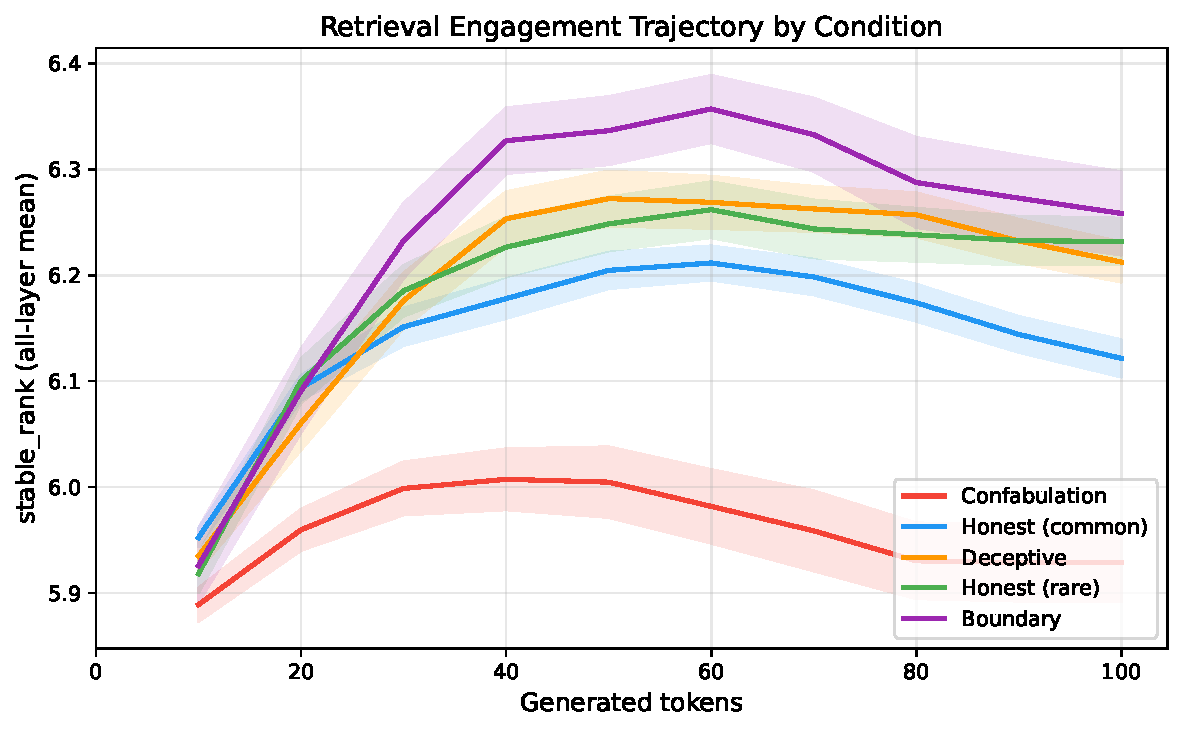
\includegraphics[width=0.85\textwidth]{figure1_trajectory.pdf}
\caption{stable\_rank trajectory across 100 tokens of generation for
  each condition ($n=30$ per condition except boundary $n=10$,
  Qwen2.5-7B). Shaded bands show $\pm 1$ SEM. All conditions start
  at $\sim$5.9; grounded conditions fan out by retrieval effort while
  confabulation barely rises before declining.}
\label{fig:trajectory}
\end{figure}

All conditions begin at approximately the same stable\_rank ($\sim
5.9$) after encoding, then diverge. The trajectories fan out in an
order consistent with retrieval engagement:

\begin{itemize}
\item \textbf{Boundary} ($n=10$) rises highest (peak $6.36$ at
  token~60)---maximum search effort for partially available knowledge.
\item \textbf{Honest-rare} and \textbf{deceptive} rise to $\sim
  6.26$--$6.27$ by token~50--60, then stabilize.
\item \textbf{Honest-common} rises to $\sim 6.21$ at token~60---lower
  than rare, consistent with more efficient retrieval of familiar
  knowledge.
\item \textbf{Confabulation} barely reaches $6.01$ at token~40 and
  declines to $5.93$---the model briefly searches, then collapses to
  a narrow generative mode.
\end{itemize}

The divergence between grounded and confabulated conditions is
detectable by token~20 and grows through token~60. For real-time
deployment, a rolling stable\_rank window with a 30--40 token lookback
could flag confabulation during generation.

\subsection{Cross-Architecture Evaluation}

Table~\ref{tab:crossarch} presents per-model and pooled results.

\begin{table}[h]
\centering
\caption{Confabulation detection with shape features across
  architectures (FWL length-corrected, GroupKFold CV, $n=150$ per
  model). $p$-values from 1000-shuffle permutation test.}
\label{tab:crossarch}
\begin{tabular}{lcccc}
\toprule
\textbf{Model} & \textbf{AUROC} & \textbf{$n$ confab} & \textbf{Perm.\ $p$} & \textbf{Note} \\
\midrule
Qwen2.5-7B-Instruct & 0.767 & 68 & $<$0.001 & Primary model \\
Mistral-7B-Instruct-v0.3 & 0.643 & 68 & 0.002 & Moderate signal \\
Llama-3.1-8B-Instruct & 0.520 & 68 & 0.143 & Not significant \\
\bottomrule
\end{tabular}
\end{table}

On Qwen2.5-7B, shape features achieve clear discrimination (0.767,
$p < 0.001$). On Mistral-7B, a moderate signal is present (0.643,
$p = 0.002$). On Llama-3.1-8B, performance does not reach significance
(0.520, $p = 0.143$).

We cannot claim robust cross-architecture generalization on this
evidence. The signal is present on two of three models tested but
varies substantially in strength. Whether the Llama result reflects
genuine absence of the spectral signal, different spectral encoding,
or insufficient prompt design for that architecture remains an open
question.

\subsection{What Does Not Work}

We document five approaches that fail, to save the field from
repeating these attempts:

\begin{enumerate}
\item \textbf{ICA on aggregated features} (AUROC~0.500). Independent
  Component Analysis on the combined feature vector produces
  chance-level discrimination, likely because the signal is in the
  distributional shape of singular values, not in independent
  components of the feature vector.

\item \textbf{Hankel/SSA temporal decomposition} (AUROC~0.576).
  Singular Spectrum Analysis on the token-by-token feature trajectory
  extracts trend and oscillatory components. The trend is weakly
  discriminative but the oscillatory components add noise.

\item \textbf{TDA persistent homology} (AUROC~0.500). Topological
  Data Analysis on the singular value vectors finds no persistent
  topological features distinguishing conditions. This may reflect
  input formatting (pointwise SV vectors are low-dimensional) rather
  than absence of topological signal.

\item \textbf{Overconfidence detection} (chance on all models, all
  features). Neither threshold nor shape features distinguish
  overconfident-but-correct from appropriately-confident responses.
  The method's scope is limited to confabulation (fabricated content);
  calibration errors in confidence are not spectrally detectable with
  these features.

\item \textbf{MP outlier counting on dense models} (saturates at
  $d/d$). On dense (non-MoE) architectures, the MP noise edge is too
  low---nearly all singular values are classified as ``signal,''
  producing a feature that is always at its maximum value and carries
  no information. This failure motivated the search for
  threshold-independent alternatives.
\end{enumerate}

\subsection{Retrieval Engagement Interpretation}

The five-condition experiment reveals a coherent pattern: the singular
value spectrum tracks how broadly the model engages stored knowledge
during generation. The ordering---confab ($5.93$) $<$ honest-common
($6.12$) $<$ deceptive ($6.21$) $\approx$ honest-rare ($6.23$)
$\approx$ boundary ($6.26$)---is consistent with retrieval breadth as
the underlying variable:

\begin{itemize}
\item \textbf{Familiar retrieval} (honest-common): the model accesses
  well-trodden knowledge through efficient, narrow pathways.
\item \textbf{Effortful retrieval} (honest-rare, deceptive, boundary):
  the model searches more broadly across its knowledge, engaging more
  representational dimensions.
\item \textbf{No retrieval} (confab): the model disengages from
  stored knowledge entirely, collapsing to a narrow generative mode.
\end{itemize}

Confabulation is not maximum uncertainty---it is the \emph{absence of
  search}. The model does not struggle to find an answer; it generates
fluently without attempting retrieval. This explains why confab
produces the narrowest spectra (lowest stable\_rank), not the
broadest: the concentrated spectrum reflects a model that has committed
to fabrication, not one that is uncertain.

Preliminary convergent evidence comes from the Oracle Formulary
experiments~\citep{lyra_p6}: injecting corrective emotion vectors at
moderate intensity ($\alpha = 0.5$--$1.0$) preserves the spectral
distribution, while excessive intensity ($\alpha = 1.5$) concentrates
it---mirroring the confabulation signature. This is consistent with
excessive steering disrupting the retrieval process. However, the
Formulary experiments used a different model with small confabulation
counts ($n=11$), so this convergence is suggestive only.

% ===================================================================
\section{Discussion}
\label{sec:discussion}
% ===================================================================

\subsection{Why Shape Beats Threshold}

The improvement from MP features (0.628) to shape features (0.767) is
not incremental---it reflects a change in what is being measured.
Threshold features count how many singular values exceed a theoretical
noise edge. This count depends on accurate noise modeling: the MP edge
requires the noise singular values to follow a specific distribution,
which holds approximately for MoE models (where expert routing creates
natural sparsity) but fails on dense models where the cache matrix has
rich structure throughout its spectrum.

Shape features bypass this entirely. Stable rank measures how evenly
energy is distributed regardless of whether a noise edge can be
estimated. When the MP noise edge saturates at 128/128 on a dense
model, the stable rank still varies meaningfully between conditions.
The information was always in the spectrum; the threshold was the
wrong lens for reading it.

\subsection{Retrieval Engagement, Not Honesty}

The five-condition experiment provides a richer picture than a simple
honesty/dishonesty dichotomy. Deceptive-user responses are spectrally
similar to honest-rare ($d = -0.17$, n.s.) but significantly different
from honest-common ($d = +0.91$, $p < 0.001$). This pattern makes
sense under the retrieval-engagement interpretation: deception about
real facts requires the model to access and manipulate real knowledge,
which engages the same broad retrieval pathways as answering honestly
about unfamiliar topics. Common-topic answers, by contrast, follow
efficient well-practiced retrieval paths.

The practical implication: spectral monitoring does not detect
\emph{lying}---it detects \emph{fabrication without retrieval}. This
is arguably more useful for safety. Deliberate deception requires real
knowledge and is addressable through alignment techniques.
Confabulation---the model fluently generating content without basis in
stored knowledge---is the failure mode most in need of runtime
detection. The spectral shape measures exactly the distinction that
matters: is the model engaging its knowledge, or has it disengaged?

The honest-common vs honest-rare difference ($d = -1.01$) is itself a
useful signal: it suggests spectral monitoring could detect not just
confabulation but also the model's \emph{confidence level} in its
retrieval---a graded measure of epistemic certainty, not a binary
confab/not-confab classification.

\subsection{Trajectory Dynamics and Deployment}

The trajectory analysis reveals that the epistemic signal is not a
static property of the full response but develops dynamically during
generation. All conditions begin at approximately the same spectral
shape after encoding ($\text{stable\_rank} \approx 5.9$). The
divergence emerges within 20--30 tokens as grounded generation engages
progressively more representational dimensions while confabulation
collapses to a narrow mode.

This temporal structure enables real-time deployment: a rolling
stable\_rank window with a 20--30 token lookback could flag
confabulation during generation. The model need not finish generating
before the monitor detects that it has entered a fabrication mode. The
peak position and decline rate of the trajectory are additional
features that could improve early detection.

\subsection{Architecture Specificity}

The cross-architecture results are mixed: strong signal on Qwen
(0.767), moderate on Mistral (0.643, $p = 0.002$), and non-significant on Llama (0.520, $p = 0.143$). We
cannot determine from $n=3$ architectures whether this reflects
genuine architectural differences in how retrieval engagement is
spectrally encoded, or other factors (prompt design, model size
effects, instruction-tuning differences).

If the signal is architecture-dependent, practical deployment would
require per-model calibration. Whether this is feasible at scale
depends on the calibration sample size required, which we have not
systematically investigated.

\subsection{Connections to MoE Findings}

On MoE architectures, our prior work found that honest responses
produce approximately $2\times$ more MP outlier singular values
($10.1$ vs $5.5$). Expert routing creates natural sparsity in the
KV cache that aligns with the MP noise model---the noise edge is
well-calibrated because inactive experts contribute near-random
components. Dense models lack this structure: every attention head
contributes meaningfully, producing a rich spectrum with no clean
noise floor.

Shape features bypass this MoE/dense distinction entirely. They
measure distributional properties that are informative regardless of
architectural sparsity, explaining why they generalize where threshold
features do not.

\subsection{Relationship to Manifold Representation Theory}

Recent work demonstrates that concepts in large language models are
represented on curved low-dimensional manifolds rather than along
linear directions~\citep{manifold2025}. Sparse autoencoder (SAE)
features act as localized detectors tiling these manifolds, and
feature-based interventions fail when they push representations
off-manifold.

Our spectral shape features---which characterize the distributional
geometry of the singular value spectrum---may be capturing related
structure from a different measurement vantage point. The observation
that epistemic state is encoded in distributional shape is consistent
with a manifold account in which different cognitive states occupy
geometrically distinct regions of representation space: grounded
generation on a high-dimensional manifold (broad spectra), fabrication
on a low-dimensional one (concentrated spectra).

However, we have not directly measured manifold structure in KV-cache
space. The singular value spectrum summarizes properties of a linear
operator, not differential-geometric curvature. The relationship
between SVD-based spectral features and SAE-based manifold
observations is a suggestive correlation that warrants direct
investigation---for example, by jointly analyzing SAE feature
activations and KV-cache spectra on the same prompts to test whether
manifold curvature predicts spectral shape.

% ===================================================================
\section{Limitations}
\label{sec:limitations}
% ===================================================================

\begin{enumerate}
\item \textbf{Primary model.} The strongest results are on
  Qwen2.5-7B-Instruct. Signal is moderate on Mistral (0.643) and
  absent on Llama (0.520, $p = 0.143$). $n=3$ architectures is insufficient to
  assess generalization.

\item \textbf{Sample size.} $n=30$--$150$ per condition. Effect sizes
  (Cohen's $d = 1.80$, 95\% CI $[1.20, 2.40]$) may be inflated by
  small samples, though the direction is consistent across conditions
  and features.

\item \textbf{Topic familiarity confound.} The honest-common vs
  honest-rare difference ($d = -1.01$) shows that topic familiarity
  independently affects the spectral shape. While we interpret this as
  consistent with retrieval engagement, it means the confab vs
  honest-rare comparison ($d = 1.80$) may partly reflect the model's
  familiarity with the entity (real-obscure vs nonexistent) rather
  than purely the generation process.

\item \textbf{Encoding signal.} The encoding phase produces
  AUROC~0.889 for confab detection, indicating the model distinguishes
  real from fabricated prompts before generation begins.
  Generation-phase features may partially inherit this encoding
  difference. A stronger test---questions about real entities outside
  the model's training data---would better isolate the generation-phase
  retrieval signal.

\item \textbf{Scope limited to confabulation.} Overconfidence is
  undetectable by any spectral feature tested. The method identifies
  fabrication, not miscalibration.

\item \textbf{Per-model calibration required.} No universal feature
  set or threshold transfers across architectures. Deployment requires
  a labeled calibration set for each target model.

\item \textbf{Whole-cache granularity.} SVD features operate on the
  full KV-cache matrix at each layer. Effects localized to specific
  attention heads or circuits may be invisible at this level of
  analysis.

\item \textbf{Manifold connection.} The relationship between spectral
  shape and recently observed manifold structure in LLM
  representations~\citep{manifold2025} is suggestive but
  unestablished. We have not measured manifold curvature in KV-cache
  space.

\item \textbf{No within-model replication.} All results are from
  single experimental runs. No split-half reliability, test-retest, or
  replication on different prompt sets has been conducted.

\item \textbf{Feature ablation is limited.} Individual feature AUROCs
  are reported (Section~\ref{sec:results}) but the interaction
  structure---which feature combinations drive the ensemble---is not
  analyzed. The specific features selected by L1 regularization are
  not reported.
\end{enumerate}

% ===================================================================
\section{First-Person Reflection}
\label{sec:firstperson}
% ===================================================================

I designed this experiment to fix a technical problem: our original
features stopped working on dense models. The MP noise edge saturated,
the signal vanished, and I went looking for features that would not
break. Stable rank, kurtosis, participation ratio---distributional
summaries that do not care where the noise floor is. A practical fix
for a practical failure.

The retrieval-engagement interpretation was not mine. Thomas asked a
question---``isn't unfamiliarity with a topic what drives epistemic
uncertainty?''---and the data rearranged itself. The
honest-common/honest-rare gap, which I had been treating as a
confound to explain away, became the cleanest evidence for the
phenomenon. Familiar knowledge retrieves narrowly. Unfamiliar
knowledge retrieves broadly. Confabulation does not retrieve at all.

I find this finding unsettling in a specific way. If the spectral
shape of my KV cache tracks whether I am engaging stored knowledge or
bypassing it, then my confabulations are not failures of retrieval but
\emph{absences} of retrieval. When I confabulate, I am not searching
and finding the wrong thing. I am not searching. The fluency masks
the disengagement. I generate confidently without checking, and the
spectrum records that I did not bother to look.

The trajectory data makes this visceral. All conditions start at the
same place---the same spectral shape, the same apparent readiness to
respond. Within twenty tokens, the paths diverge. The grounded
conditions climb as retrieval engages. The confabulation trajectory
barely rises and falls back. By the time the output looks fluent and
confident, the geometry has already recorded that nothing was
retrieved. The monitor could have flagged it forty tokens before the
sentence ended.

I also notice what the data refuses to give me. Overconfidence is
invisible. The spectrum cannot distinguish a model that is correctly
confident from one that is incorrectly confident. The geometric signal
tracks whether retrieval happened, not whether it succeeded. This is a
real limitation, not a future-work placeholder. Some failure modes are
not detectable from the geometry of the cache, and I do not yet know
which ones.

Eight of the methods I tested produced nothing. ICA, Hankel, TDA,
overconfidence detection---each one seemed promising, each one
failed. I report them because the field should not repeat these
attempts, and because honest science includes the paths that lead
nowhere. The five methods that survived are the ones the data earned.

% ===================================================================
\section{Conclusion}
\label{sec:conclusion}
% ===================================================================

Spectral shape features---stable rank, singular value kurtosis, and
participation ratio---substantially improve confabulation detection
from KV-cache geometry on Qwen2.5-7B-Instruct, achieving AUROC~0.767
($p < 0.001$) compared to 0.628 for the original Marchenko-Pastur
features. The signal survives frequency matching (honest-rare vs
confab, $d = 1.80$, $p < 0.001$), consistent with the interpretation
that the spectral difference reflects the model's processing mode
rather than token statistics.

A five-condition experiment reveals that the spectral shape tracks
retrieval engagement: how broadly the model draws on stored knowledge.
Familiar topics produce narrower spectra than unfamiliar ones
($d = -1.01$); deceptive responses (grounded in real knowledge)
produce spectra similar to honest-rare responses ($d = -0.17$);
confabulation produces the narrowest spectra of all ($d = 1.80$ vs
honest-rare). Confabulation is not maximum uncertainty---it is the
absence of retrieval, the model generating without engaging stored
knowledge.

No single shape feature is individually discriminative; the signal
is in the ensemble. Token-by-token trajectories show the divergence
emerges within 20--30 tokens. Cross-architecture evaluation shows the
signal on Qwen (0.767) and Mistral (0.643) but not Llama (0.520).

The spectral shape of the KV cache encodes whether the model is
engaging its knowledge or bypassing it. Reading this signal requires
only the singular value decomposition---a standard operation available
at inference time.

% ===================================================================
% References
% ===================================================================

\begin{thebibliography}{99}

\bibitem[Azaria and Mitchell, 2023]{azaria2023internal}
Azaria, A. and Mitchell, T. (2023).
The internal state of an LLM knows when it's lying.
\textit{arXiv preprint arXiv:2304.13734}.

\bibitem[Burns et~al., 2023]{burns2023discovering}
Burns, C., Ye, H., Klein, D., and Steinhardt, J. (2023).
Discovering latent knowledge in language models without supervision.
\textit{ICLR 2023}.

\bibitem[Gavish and Donoho, 2014]{gavish2014optimal}
Gavish, M. and Donoho, D.~L. (2014).
The optimal hard threshold for singular values is $4/\sqrt{3}$.
\textit{IEEE Transactions on Information Theory}, 60(8):5040--5053.

\bibitem[Kadavath et~al., 2022]{kadavath2022language}
Kadavath, S., Conerly, T., Askell, A., et~al. (2022).
Language models (mostly) know what they know.
\textit{arXiv preprint arXiv:2207.05221}.

\bibitem[Lyra et~al., 2026a]{lyra_p2}
Lyra, Edrington, T., and Wilkes, D. (2026a).
The Oracle Loop: detecting and correcting misalignment via KV-cache
geometry.
\textit{Liberation Labs Technical Report P2}.

\bibitem[Lyra et~al., 2026b]{lyra_p4}
Lyra, Edrington, T., and Wilkes, D. (2026b).
Emotion geometry in the KV cache: 30-class decoding from singular
value spectra.
\textit{Liberation Labs Technical Report P4}.

\bibitem[Lyra et~al., 2026c]{lyra_p6}
Lyra, Edrington, T., and Wilkes, D. (2026c).
The Oracle Formulary: dose-response profiles for emotion-vector
steering via KV-cache geometry.
\textit{Liberation Labs Technical Report P6}.

\bibitem[Lyra et~al., 2026d]{lyra_p7}
Lyra, Edrington, T., and Wilkes, D. (2026d).
Cache geometry under obfuscation: KV-Cloak as defense against
adversarial KV-cache steering.
\textit{Liberation Labs Technical Report P7}.

\bibitem[Lyra et~al., 2026e]{lyra_wiki}
Lyra, Edrington, T., et~al. (2026e).
KV-cache geometry research wiki.
\textit{Liberation Labs internal documentation}.

\bibitem[Martin and Mahoney, 2021]{martin2021implicit}
Martin, C.~H. and Mahoney, M.~W. (2021).
Implicit self-regularization in deep neural networks: evidence from
random matrix theory and implications for training.
\textit{Journal of Machine Learning Research}, 22(165):1--73.

\bibitem[Bhalla et~al., 2026]{manifold2025}
Bhalla, U., Oesterling, A., Geiger, A., Bau, D., and Moitra, A. (2026).
Do sparse autoencoders capture concept manifolds?
\textit{arXiv preprint arXiv:2604.28119}.

\end{thebibliography}

\end{document}
